\subsection{Algorithm description} \label{sec:algorithm-desc}

After the \projname{} has completed its initial 360 degree search and stored the information about the nearby objects, it is time to calculate a route between said objects. Due to the limited power and calculation speed of the LEGO NXT brick it is necessary to find an efficient algorithm that is fast and does not take a lot of computational power and space. 

The shortest route between the object can be brute forced by trying out every single possible route between the start position and all of the objects. This would have a calculation time of $\mathcal{O}(n!)$, which means that every object added greatly increases the running time. This gives the robot problems when calculating a shortest route, if the amount of objects exceed a certain number. If there are 9 objects, the number of different paths to check exceeds 360000. 

A more time efficient, but less effective, algorithm is the NN-algorithm. The algorithm calculates a route based on which objects are closest together. This means that the distance to all the points are calculated from the starting point and the shortest distance is chosen. This is then repeated from the new point, but this time it does not calculate from any previously visited points.

A very simple algorithm, that uses very little calculation, is the next-in-view algorithm. This was the first algorithm to be implemented on the \projname{} due to its simplicity. With this algorithm, the robot starts turning towards either right or left, stopping at the first object it detects. It then moves out to collect this object, and then starts turning towards the same direction again, thus always picking up the next object that comes into its view, hence the name of the algorithm. This algorithm has a number of issues connected to it, which may reduce its performance, however in smaller cases with less than ten objects, its completion speed is close to the NN-algorithm.

\begin{figure}[H]
     \center\frame{{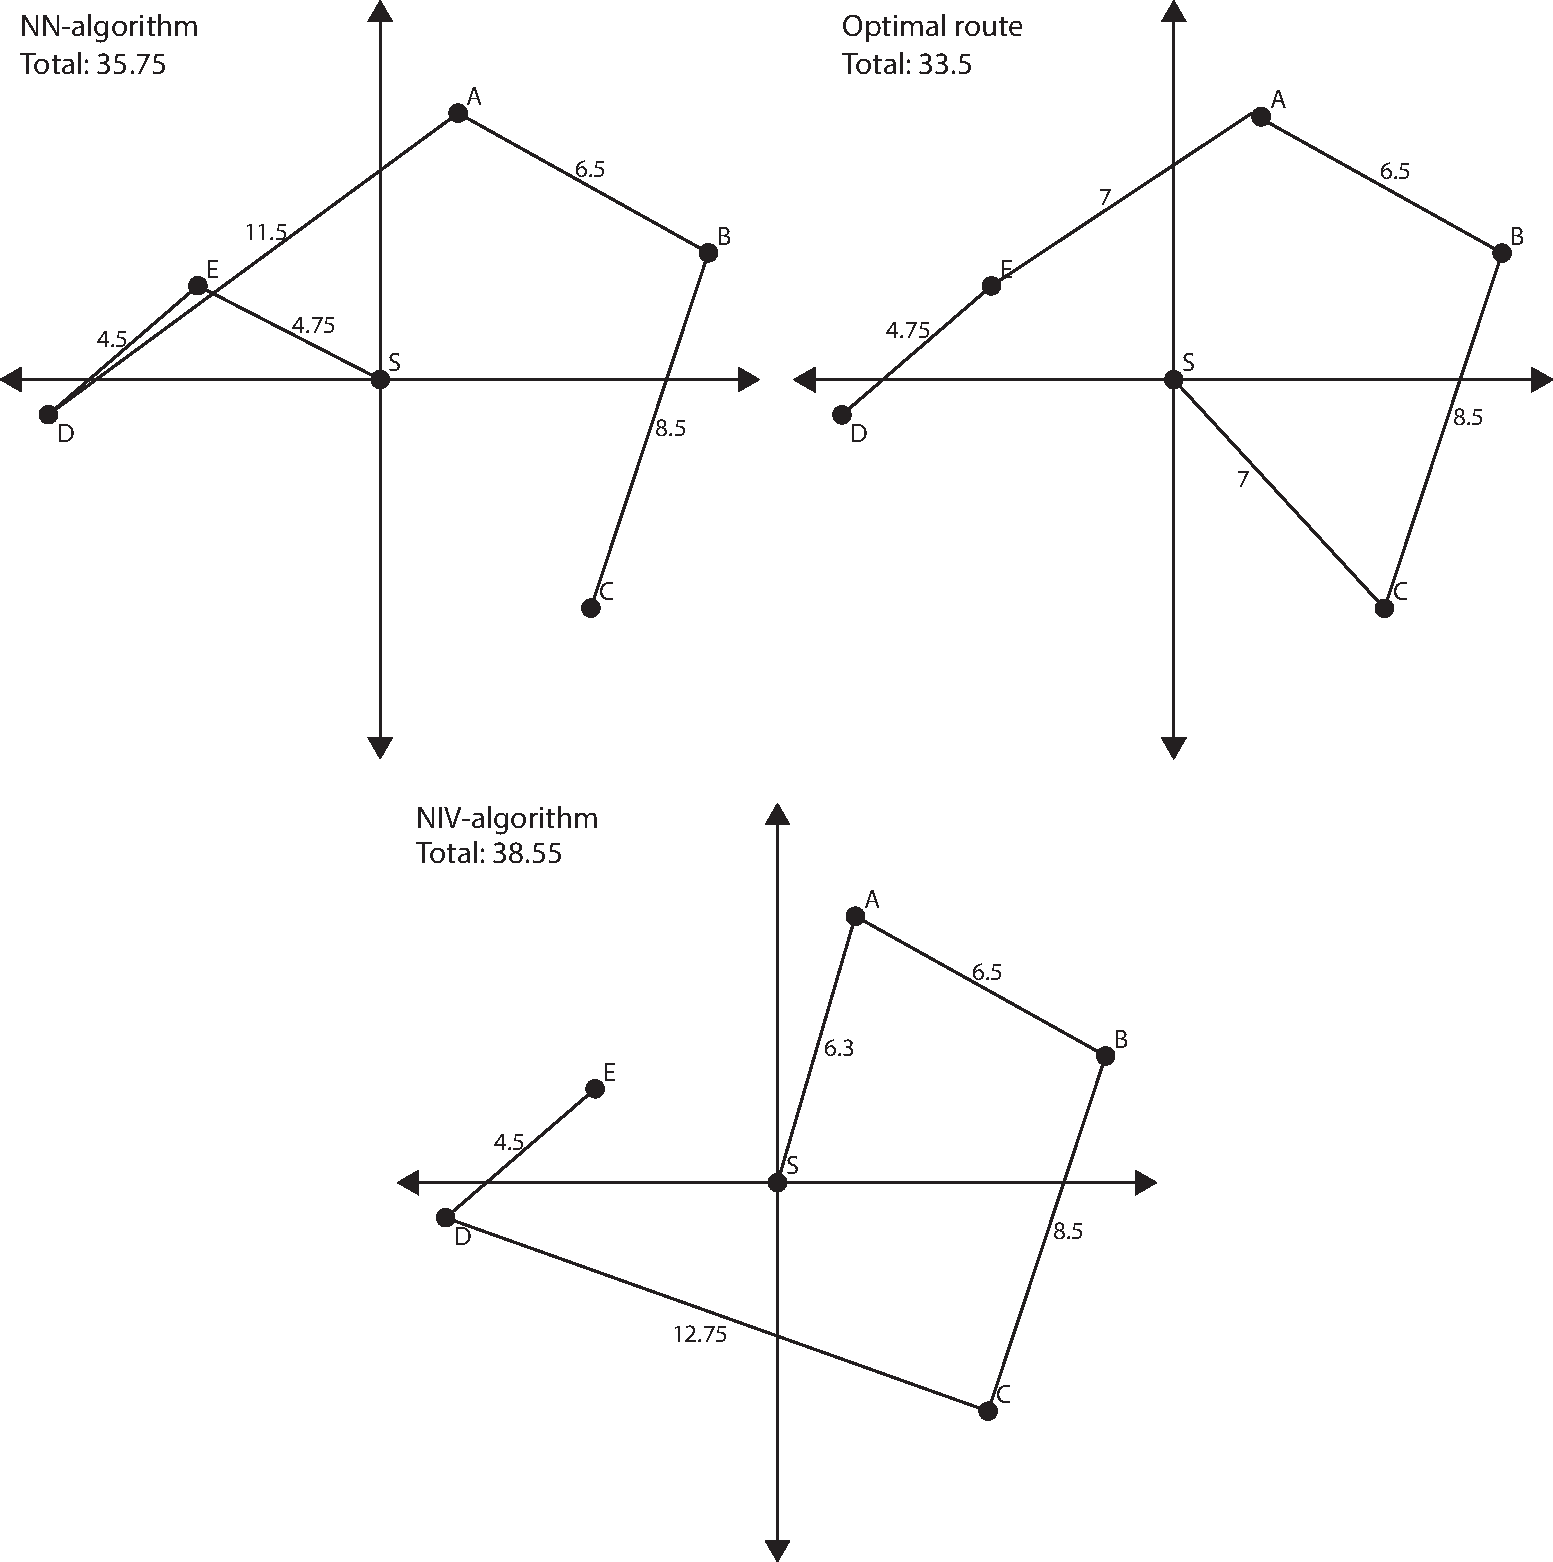
\includegraphics[width=\textwidth]
     {graphics/AlgorithmExamples2.pdf}}}
     \caption{\label{fig:algorithm-example} Example of the NN-algorithm, the optimal algorithm, and next-in-view algorithms.}
\end{figure}

\figref{fig:algorithm-example} shows three solutions to the problem. The top right graph is the optimal solution, which is only used to compare the results from the two other algorithms. Top left is the NN-algorithm, and in the bottom the next-in-view algorithm. The robot starts its route at position \emph{S}. The objects are named in order as they are first detected. The algorithms result in the routes shown on the figure.

The different solutions in \figref{fig:algorithm-example} have following lengths:
\begin{itemize}
\item Optimal: 33.5 units
\item NN-algorithm: 35.75 units
\item Next-in-view: 38.55 units
\end{itemize}

In the average case, the difference between the NN-algorithm and the next-in-view solutions would be larger if there were more objects to consider. However for these smaller cases, the difference is almost negligible. It should be noted, that this does not describe the time spent, only the distance travelled: rotation to scan for objects, for both algorithms, will also take different amounts of time depending on the case. This is not accounted for here.

Due to the limitations of the LEGO NXT brick and the complexity of the problem, finding the optimal solution was ruled out as a possibility. Instead, the NN-algorithm was initially selected to calculate the route for the \projname{}. This algorithm does not always result in the most optimal route, but when the calculation speed and actual running speed is considered, it is arguably faster in the average case. However, as previously mentioned, this algorithm was not implemented. This was the result of inaccurate hardware: the ultrasonic sensor was not able to detect objects with enough precision, that the \projname{} could accurately calculate any useful information based on the data.

Due to this limitation, the \emph{next-in-view} algorithm was chosen for implementation. The simplicity of the algorithm, as well as the fact that it takes the inaccurate sensor input into account, made it the obvious choice. And as previously mentioned in \secref{sec:nn-algorithm}, the distance difference of the two algorithms are nearly insignificant.
